\section{Familiarisering af værten}
\label{FamiliariseringSocialAccept}
% 
Familiariseringen af værten er bygget op så de gradvist bliver introduceret til både gestikker og hints. Inden selve familiariseringen påbegyndes introducerer testleder 1 værten i hvad der kommer til at foregå. Instruktionerne fremgår af \autoref{app:InstruktionerVaert}. Derefter starter testleder 1 videoen, der er specielt redigeret til familiariseringen og som vil blive uddybet i \fullref{VideooptagelseSocialAccept}. I videooptagelsen bliver testpersonen ad to omgange præsenteret for de udvalgte gestikker, hvor der forinden hver gestik præsenteres angives hvilken funktion gestikken tilhører. Efterfølgende præsenteres testpersonen for gestikkerne igen, men denne gang er det uden informationen om hvilken funktion gestikken tilhører. Til slut i videooptagelsen præsenteres testpersonerne endnu en gang for hver gestik, uden information om den tilhørende funktion, da testleder 1 spørger testpersonerne om hvilken funktion den specifikke gestik tilhører. Når testpersonerne har gennemgået videooptagelsen, så forklarer testleder 1 den næste del af familiariseringen; testpersonerne får lov til at gengive gestikkerne til musik, som startes af testleder 2 inde fra kontrolrummet. Testpersonerne får i den forbindelse mulighed for at gengive de udvalgte semaforiske gestikker samt stille opklarende spørgsmål, hvis de har behov for det. Når testpersonen er blevet kendt med gestikkerne, forklarer testleder 1 hvilke hints der bliver præsenteret samt hvordan testpersonen skal reagerer på disse. Testleder 1 signalerer til testleder 2 at afspilningslisten for familiariseringen skal startes, således at testpersonen har mulighed for at blive bekendt med de forskellige hints og i den forbindelse hvordan de skal reagerer på dem. Når testpersonen giver udtryk for at have forstået koblingen mellem hints og reaktion, så forlader testleder 1 lokalet, hvorefter afspilningslisten startes forfra. I løbet af de syv musiknumre, som udgøre afspilningslisten vil testpersonerne præsenteres for 18 hints, hvis rækkefølge fremgår af \autoref{tab:PraesentationsraekkefoelgeHints}.

For at sikre at testpersonerne efterfølgende er i stand til både at interagere med musikanlægget og samtidig føre samtalen med gæsten, så vil familiariseringen forlænges i tilfælde af at testpersonerne begår tre eller flere fejl i gestikuleringen. Udover en fejl i gestikuleringen så betragtes det ligeledes som en fejl hvis testpersonerne ikke formår, at reagerer på hintet inden de 30 sekunder er gået. Da hintet for at pause og starte musikken er en telefonopringning, så er der både mulighed for, at testleder 2 kan instruerer testpersonerne yderligere hvis der er behov for det og for at testpersonen selv kan stille opklarende spørgsmål. Når testpersonen har gennemgået de 18 hints, så er familiariseringen færdig.\blankline
%
På baggrund af \fullref{TestresultaterVolumen} hvor nogle testpersoner gav udtryk for, at bevægelsen i gestik-par 2, til at skrue op og ned for musikken, så ubehagelig og ukomfortabel ud, vælges det, at foretage nye videooptagelser. I den forbindelse vælges det, at optage de tre gestik-par fra ny så de alle har det samme udtryk både i forhold til lokation, vinkel på videokameraet, demonstratorens beklædning og andre karakteristikas. Ydermere vurderes det, at demonstratoren denne gang skal sidde ned og gengive gestikkerne for, at værten præsenteres for gestikkerne i noget der minder om en dagligstue. I \autoref{app:VideooptagelseSocialAccept} vil videoptagelsen til familiariseringen uddybes. 
% 
\subsection{Videooptagelse}
\label{VideooptagelseSocialAccept}
%
Videooptagelsen til familiariseringen af værten blev optaget i B5-106 Målerum Q med et KAMERA på et stativ, videokameraet optager både billede og lyd og optagelserne er taget med en 45$^\circ$'s vinkel i et halvnært perspektiv samt et neutralt ansigtsudtryk, ligesom det er tilfældet i \fullref{VideooptagelserValgAfGestikker}. På \autoref{fig:Test2Pause} illustreres hvordan optagelsen er foretaget. 
%
\begin{figure}[H]
	\centering
	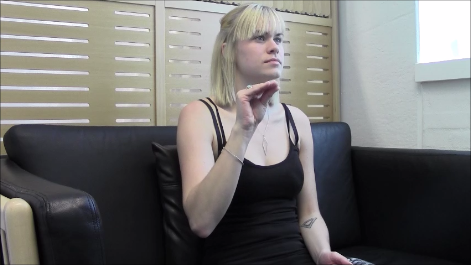
\includegraphics[resolution=300,width=0.9\textwidth]{FlowdiagramTest2/Test2_pause}
	\caption{Illustration af hvordan optagelsen foretages, med en 45$^\circ$'s vinkel i et halvnært perspektiv og hvor demonstratoren er siddende med et neutralt ansigtsudtryk.}
	\label{fig:Test2Pause}
\end{figure}
\noindent
%
Under optagelsen afspilles der musik fra en computer. Musiknummeret til at pause og starte musikken er "Love you can save it all" fra Andra (2016), musiknummeret der skiftes til, når der skiftes sang er "How would you feel" fra Ed Sheeran (2017) og musiknummeret til at skrue op og ned for musikken er "New man" fra Ed Sheeran (2017). Disse musiknumre er valgt ud fra de samme kriterier, som er beskrevet i \fullref{VideooptagelserValgAfGestikker}.

Optagelsen redigeres i Windows Movie Maker version 2012. På \autoref{fig:FlowdiagramFami} illustreres rækkefølgen på de skærmbilleder, som videoen består af.      
%
\begin{figure}[H]
	\centering
	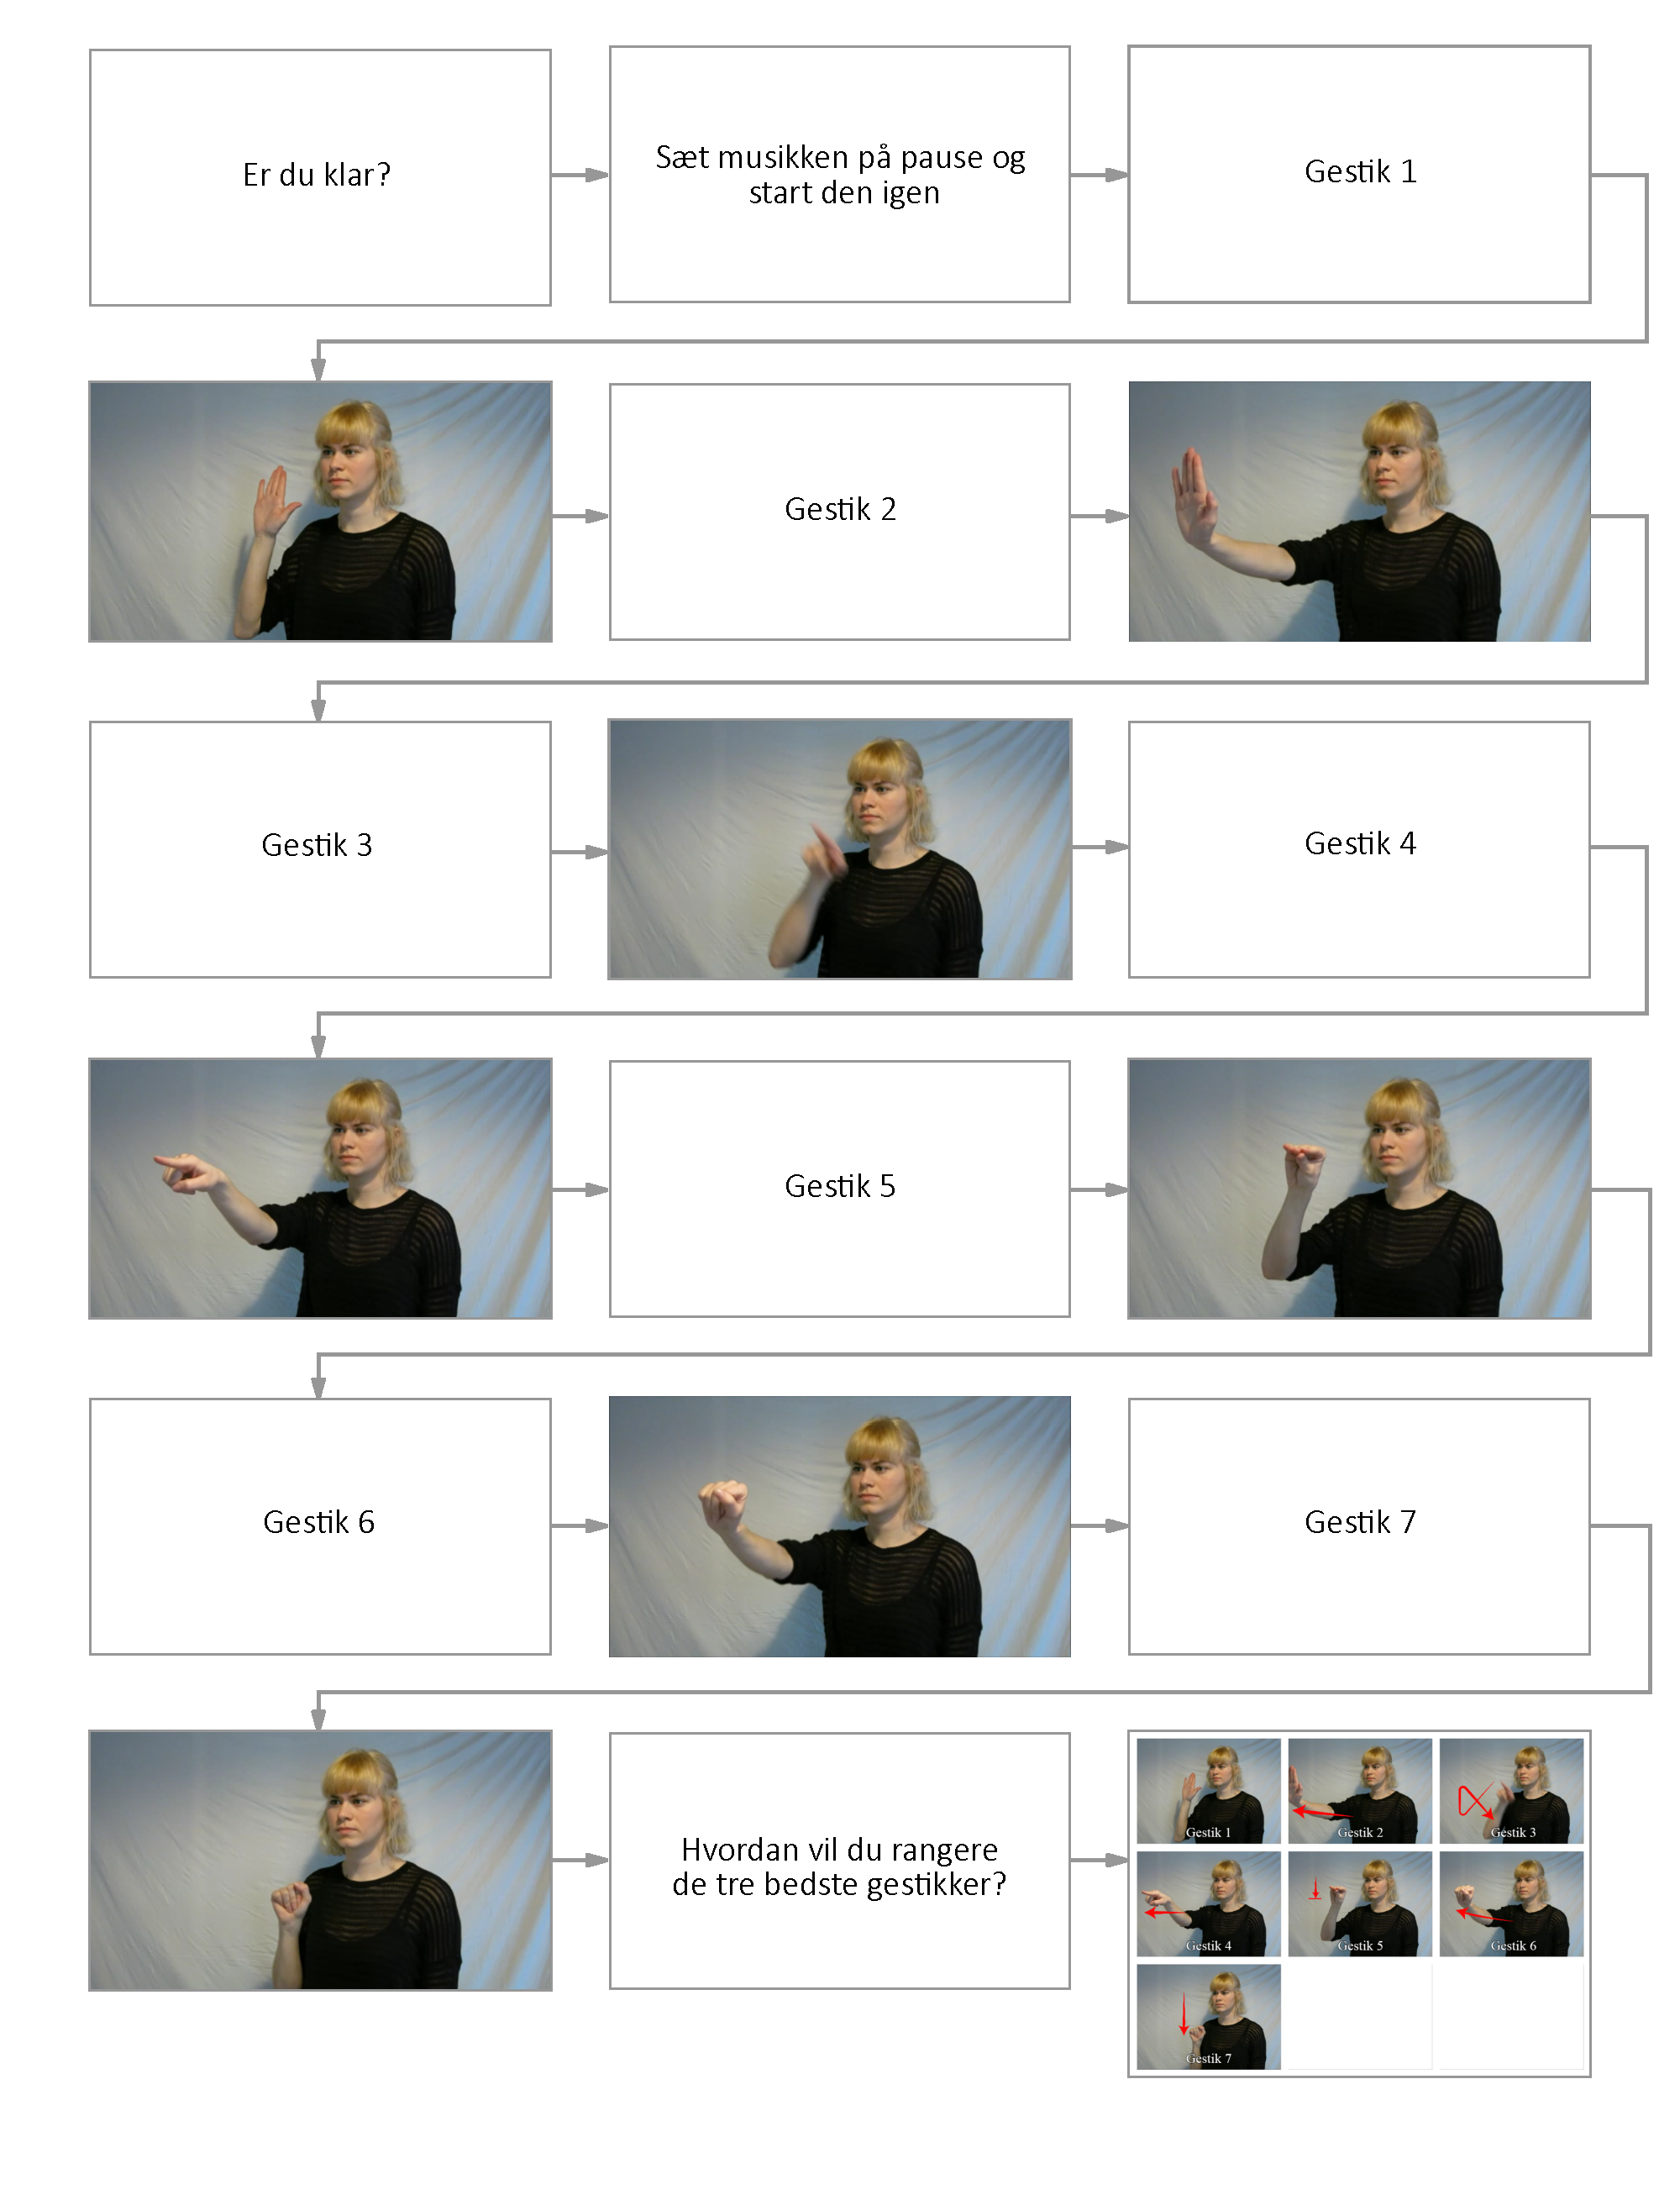
\includegraphics[resolution=300,width=\textwidth]{Flowdiagram/FlowdiagramPauseogStart}
	\caption{Illustration af hvilke skærmbilleder, der indgår i videoen til familiariseringen af værten.}
	\label{fig:FlowdiagramFami}
\end{figure}
\noindent
%
Det første skærmbillede testpersonerne præsenteres for består af teksten: \textit{Er du klar?} og præsenteres i 3 sekunder, før skærmbilledet med teksten: \textit{Sæt musikken på pause og start den igen} præsenteres i tre sekunder. Teksten på det andet skærmbillede tilpasses afhængigt af hvilken funktion, der præsenteres. Første gang testpersonerne præsenteres for de tre tekster, som angiver funktion, er varigheden tre sekunder kontra når testpersonerne præsenteres for de tre tekster anden gang, hvor varigheden sættes ned til to sekunder. Når testpersonerne er blevet præsenteret for hvilken gestik, der skal bruges til at skrue op og ned for musikken, er der et blankt skærmbillede på to sekunder, inden testpersonerne præsenteres for gestikkerne uden information omkring funktion. De to blanke skærmbilleder før og efter optagelsen af gestik-par 5 til at skifte musiknummer, varer et sekund. Efter optagelsen af gestik-par 2 til at skrue op og ned for musikken præsenteres endnu et blankt skærmbillede på to sekunder, hvorefter testpersonen er nået til den del af familiariseringen hvor de præsenteres for gestikkerne og derefter skal angive hvilken funktion gestikken tilhører. Skærmbilledet med teksten: \textit{Hvilken funktion havde gestikken?} præsenteres i syv sekunder og teksten tilpasses afhængigt af funktion. Alt i alt varer videoptagelsen 3 minutter og 16 sekunder. 



